\vspace{0.25cm}\\
\begin{minipage}{0.32\textwidth}
    \centering
    \vspace{0.1cm}
    \begin{figure}[H]
    \begin{tikzpicture}[level distance=1.5cm,
        level 1/.style={sibling distance=3cm},
        level 2/.style={sibling distance=1.5cm},
        every node/.style = {minimum width = 2em, draw, circle}
        ]
        \node[fill=blue!70] {5}
            child {node {3}
                child {node {1}}
                child {node {4}}
            }
            child {node[fill=!10!orange] {6}
                child {edge from parent[draw = none]}
                child {node {8}
                    child {node {7}}
                    child {node {9}}
                }
            };
    \end{tikzpicture}
    \caption{Find the node you want to remove (orange) and that node's parent (blue)}
    \label{fig:onesubtree-1}
    \end{figure}
\end{minipage}
\hfill
\begin{minipage}{0.32\textwidth}
    \centering
    \begin{figure}[H]
    \begin{tikzpicture}[level distance=1.5cm,
        level 1/.style={sibling distance=3cm},
        level 2/.style={sibling distance=1.5cm},
        every node/.style = {minimum width = 2em, draw, circle}
        ]
        \node[fill=blue!70] (P) {5}
            child {node {3}
                child {node {1}}
                child {node {4}}
            }
            child {node[fill=!10!orange] (R) {6}
                child {edge from parent[draw = none]}
                child {node (C) {8}
                    child {node {7}}
                    child {node {9}}
                }
            };
        \draw (P) to [bend left=40] (C);

        % I can't figure out how to remove the edge from the tree so we're 
        % just going to use some "whiteout"
        \foreach \x in {0,...,4}
            \draw[thick, white!100] (P) to (R);
    \end{tikzpicture}
    \caption{Set \lstinline|parent.right| to the root of the node we want to remove's subtree.}
    \label{fig:onesubtree-2}
    \end{figure}
\end{minipage}
\hfill
\begin{minipage}{0.3\textwidth}
    \centering
    \vspace{0.75cm}
    \begin{figure}[H]
    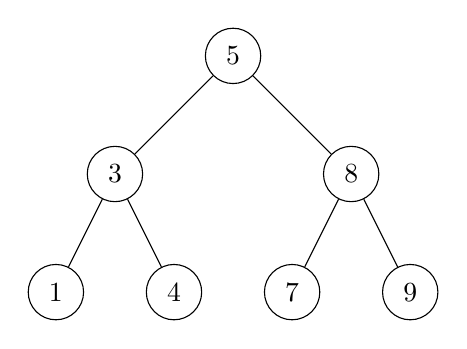
\begin{tikzpicture}[level distance=1.5cm,
        level 1/.style={sibling distance=3cm},
        level 2/.style={sibling distance=1.5cm},
        every node/.style = {minimum width = 2em, draw, circle}
        ]
        \node {5}
            child {node {3}
                child {node {1}}
                child {node {4}}
            }
            child {node {8}
                child {node {7}}
                child {node {9}}
            };
    \end{tikzpicture}
    \vspace{0.9cm}
    \caption{Set the node we  want to remove's reference to it's subtree is \lstinline|null|, thus removing it from the tree}
    \label{fig:onesubtree-3}
    \end{figure}
\end{minipage}
\vspace{0.25cm}\\

The second case, where the node we want to remove has a right or left subtree,
is still relatively straight forward. As with the first step we begin by
finding the node we want to remove and it's parent
(Figure~\ref{fig:onesubtree-1}).  We then take the right pointer of the parent
and short-circut the tree by updating it to point to root of the node we want 
to remove's existing subtree (Figure~\ref{fig:onesubtree-2}). Now, at this point
the node is no longer reachable but it is still attached to the graph. In order
to totally remove it we must set the reference from the node we want to remove
to the root of it's subtree equal to \lstinline|null| (Figure~\ref{fig:onesubtree-3}).
